\begin{center}

  \begin{tabular}{rp{16cm}lp{20cm}}%{rl}

  % after \\: \hline or \cline{col1-col2} \cline{col3-col4} ...

  论文地址:& \href{http://yhwu.me/publications/dysat_wsdm20.pdf}{http://yhwu.me/publications/dysat\_wsdm20.pdf} \\
  来源:& WSDM, 2020\\
  作者:& Aravind Sankar, Yanhong Wu, et al. \\
  源码:& \href{https://github.com/aravindsankar28/DySAT}{DySAT} \\

%  slides:& \href{http://yunshengb.com/wp-content/uploads/2017/03/nips_2018_r2l_workshop_talk.pdf}{{\footnotesize Convolutional Set Matching for Graph Similarity}}\\

  关键词:& \textbf{self-attention, representation learning, dynamic graphs} \\

  写于:& \date{2021-03-02}

  \end{tabular}

\end{center}

该论文\cite{sankar2020dysat}解决的是动态图中的结点表征问题。论文提出了DySAT(Dynamic Self-Attention),以自注意力机制捕捉动态图的结构的动态性。DySAT分别从两个方面捕捉动态性:structural neighborhoods和temporal dynamics,并且使用多头注意力来捕捉多方面的动态性。

\paragraph{问题定义}
论文中使用图序列来表示动态图。关于动态图的建模,在这里插一句。

\subparagraph{dynamic graph}
动态图通常由两种建模方式:图序列(graph snapshots)和基于带时间戳的事件的图(time stamped events,类似于流图)。本质上来看这两种建模方式是等价的,是可以互相转化的。但是不同的建模形式针对这不同的应用场景。snapshot形式的动态图,直观上强调的整体性,图中结点/边的变化是为了整体的图而服务的,这种情况下我们更多的考虑的是作为一个整体的图的应用场景,例如在场景识别中、对图进行分类的任务中。而timestamped形式的动态图,对整体的考虑可能会不是那么强,更强调的是图中结点/边以及这些变化对任务的影响。

作者采用的是snapshots形式的动态图$\mathbb{G} = \{\mathcal{G}^1, ..., \mathcal{G}^T\}$。其中$T$是时间步的数量,$\mathcal{G}^t = (\mathcal{V}, \mathcal{E}^t)$。显然,该论文中动态图的结点是不变的,即\tbc{red}{不涉及结点的增加或删除}。最终的目标就是学习图中每个结点在任意时间$t$时的表征。

\paragraph{DySAT思路}
\begin{figure}[h]
	\centering
	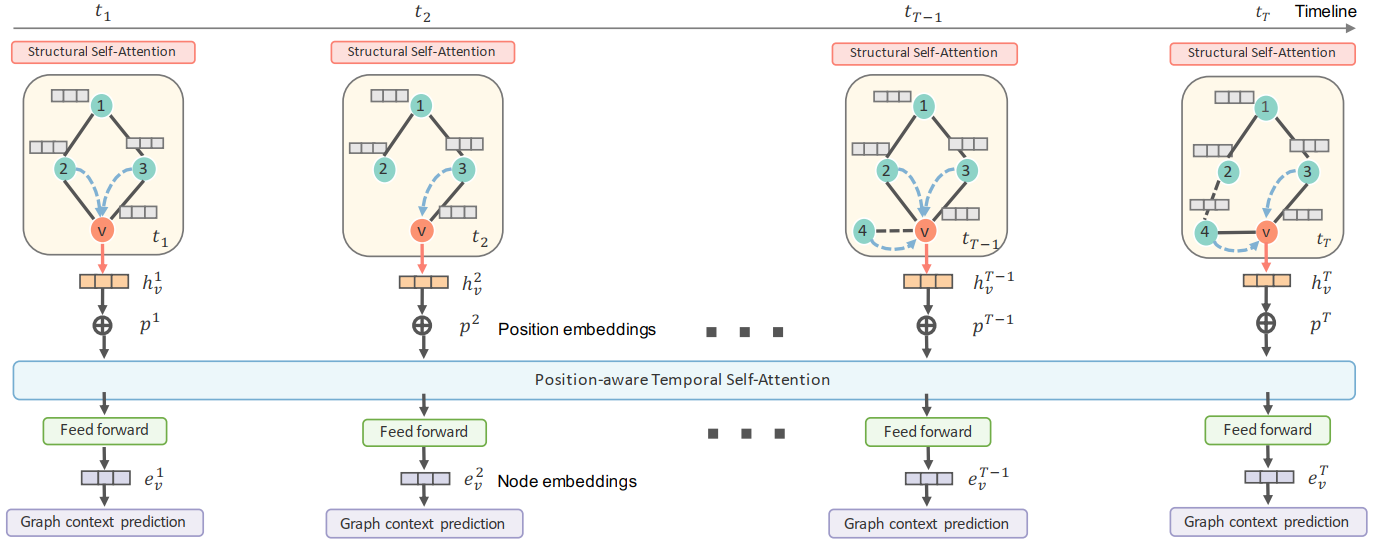
\includegraphics[width=.8\textwidth]{pics/DySAT.png}
	\caption{DySAT}
	\label{fig:dysat}
\end{figure}
DySAT的整体框架如Fig.\ref{fig:dysat}所示。DySAT主要分为两个部分:Structural Self-Attention和Temporal Self-Attention。

\subparagraph{Structural Self-Attention}
这一部分与GAT中的注意力机制类似,想当于一个邻居结点信息汇聚层。对于每一个snapshot graph,Structural Self-Attention利用当前时刻各个结点的表征计算注意力再进行加权求和,计算公式如下:
$$
\begin{array}{c}
	z_{v}=\sigma\left(\sum_{u \in \mathcal{N}_{v}} \alpha_{u v} W^{s} x_{u}\right), \alpha_{u v}=\frac{\exp \left(e_{u v}\right)}{\sum_{w \in \mathcal{N}_{v}} \exp \left(e_{w v}\right)} \\
	e_{u v}=\sigma\left(A_{u v} \cdot \boldsymbol{a}^{T}\left[\boldsymbol{W}^{s} \boldsymbol{x}_{u} \| \boldsymbol{W}^{s} \boldsymbol{x}_{v}\right]\right) \forall(u, v) \in \mathcal{E}
\end{array}
$$

\subparagraph{Temporal Self-Attention}
这部分是为了捕捉动态图在时间上的变化模式。计算结点$v$在$t$时的表征时,将在$t$之前的$v$的表征作为temporal self-attention模块的输入,输出的是结点$v$在各个事件点的表征(此时的表征考虑了动态性),计算公式如下:
$$
\begin{array}{r}
	Z_{v}=\beta_{v}\left(X_{v} W_{v}\right), \quad \beta_{v}^{i j}=\frac{\exp \left(e_{v}^{i j}\right)}{\sum_{k=1}^{T} \exp \left(e_{v}^{i k}\right)} \\
	e_{v}^{i j}=\left(\frac{\left(\left(X_{v} W_{q}\right)\left(X_{v} W_{k}\right)^{T}\right)_{i j}}{\sqrt{F^{\prime}}}+M_{i j}\right)
\end{array}
$$
上式的形式与self-attention的形式一致。其中的$\mathbf{M} \in \mathbb{R}^{T \times T}$是一个掩码矩阵,
$$
M_{i j}=\left\{\begin{array}{ll}
	0, & i \leq j \\
	-\infty, & \text { otherwise }
\end{array}\right.
$$

通常一个注意力捕捉的是一个方面的性质,为了捕捉动态图中多个方面的动态性,作者引入了多头注意力,Structural和Temporal都引入了多头注意力机制。

为了训练模型中的参数,论文使用类似神经语言模型中的共现率来优化参数,这点与word2vec和Node2vec中的损失函数很像,损失函数如下,$P_n^t$为负采样的结点:
$$
\begin{aligned}
	L=\sum_{t=1}^{T} \sum_{v \in \mathcal{V}}\left(\sum_{u \in \mathcal{N}_{\text {walk }}^{t}(v)}-\log \left(\sigma\left(<\boldsymbol{e}_{u}^{t}, \boldsymbol{e}_{v}^{t}>\right)\right)\right.\\
	&\left.-w_{n} \cdot \sum_{u^{\prime} \in P_{n}^{t}(v)} \log \left(1-\sigma\left(<\boldsymbol{e}_{u^{\prime}}^{t}, \boldsymbol{e}_{v}^{t}>\right)\right)\right)
\end{aligned}
$$

DySAT是先进行structural self-attention再进行temporal self-attention,作者这样设计是因为:随着时间变化,图的结构是不稳定的。

\paragraph{方法解决的问题/优势}

\begin{itemize}

	\item 提出了structural和temporal self-attention来学习动态图中的结点表征
	\item 使用多头注意力机制捕捉多方面的动态性
	\item 注意力机制适用于并行

\end{itemize}

\paragraph{方法的局限性/未来方向}

\begin{itemize}

	\item 只能适用于结点不变化的动态图
	\item 以结点的共现率为损失函数引导模型的训练,这样的损失函数可能重点关注的是图的结构,对于动态性更丰富的图(如结点的特征的变化)是不够的

\end{itemize}


